\problemname{TileTraveller}

In this assignment, you extend the functionality of the TileTraveller program you implemented earlier, in Assignment 8.

We recommend that you start with the solution given on
\href{https://github.com/reykjavik-university/2023-3-T-111-PROG/blob/main/assignments/08_tile_traveller/a08p01tiletraveller/solution_code.py}{Github},
also included in the attached starter code for your convenience,
and make sure that you study it and understand how it works.

As in the first TileTraveller project, you should work on this in a group of two.
Apply pair (or tri) programming, one student programs while the other one(s) follows and comments on the code,
and then you switch roles, several times.
You should use git while you work on the project,
i.e. apply commands like
\texttt{git status},
\texttt{git log},
\texttt{git add},
\texttt{git commit},
\texttt{git push} and
\texttt{git pull}.

This is our grid of tiles, as before:

\begin{figure}[h]
    \centering
    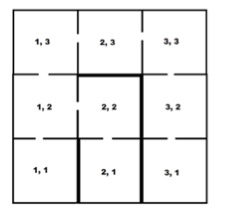
\includegraphics[width=0.33\textwidth]{grid}
    \caption{\texttt{Maze}}
\end{figure}
